%\vspace{-5pt}
\section{Experiments and Results}
\label{sec:results}
In this section, we discuss some preliminary results for the models described in
Section~\ref{sec:memoryless} evaluated on the Linux kernel source code with
2000 key tokens ($K = 2000$) and window length of 40 ($W = 40$).

\begin{table}[h]
  \centering
  \begin{tabular}{l r r r r r}
    \hline
    Method & Known & Abs. & Top 3 & Key & Pos. \\
    \hline
    x & x & x & x & x & x\\
    \hline
  \end{tabular}
  \caption{Results for Linux project}
  \label{tab:linux}
\end{table}

\begin{table}[h]
  \centering
  \begin{tabular}{l r r r r r}
    \hline
    Method & Known & Abs. & Top 3 & Key & Pos. \\
    \hline
    x & x & x & x & x & x\\
    \hline
  \end{tabular}
  \caption{Results for Twisted project}
  \label{tab:twisted}
\end{table}

We observed that among the models discussed, the Non-Linear Matrix Vector Model
gave the best accuracy (55\% accuracy as opposed to $\approx$ 45\% for Fixed
Window Weight Model and $\approx$ 50\% for Matrix Vector Model). Overall, we
found that 46\% of the windows had an output that is a key token, and 30\% had
an output that was a positional token. This underlines the importance of also
considering non-keyword tokens while doing prediction.

The accuracy of predicting the keyword tokens was {\bf 72\%}, while the accuracy
of predicting the non-keyword tokens was {\bf 29\%}. We also evaluated the
accuracy of a random predictor on the non-keyword tokens, and that achieves an
accuracy of 8\%, which is significantly lower than the accuracy achieved by our
model (29\%). Overall, the accuracy on windows with keyword/positional tokens is
{\bf 55\%}, which translates to an accuracy of 42\% over all windows (including
windows with UNKNOWN output, which if outside of the capability of our model to
predict).

Another experiment we ran was to evaluate the accuracy of the classifier in a
setting where, if the correct token is not within the top few predictions, the
user types in one or more characters to ``home in'' on the correct prediction.
Figure~\ref{fig:codeexample} shows the results for this experiment. In this
experiment, a character is colored in green if the token is correctly predicted
(i.e., top prediction) before that character is typed. It is colored in yellow
if the token is among the top 5 before typing that character, and colored in red
if the token is not among the top 5. So, for example, in the first
{\tt int} the character {\tt i} is in yellow since before typing {\tt i}, the
token {\tt int} was among the top 5. After typing {\tt i}, the top prediction
was {\tt int}, and thus the characters {\tt n} and {\tt t} are both in green. We
can see that, for example, entire sequences of code such as {\tt if (rc) return
rc;} are predicted correctly without typing anything.
\begin{figure}[h]
  \centering
  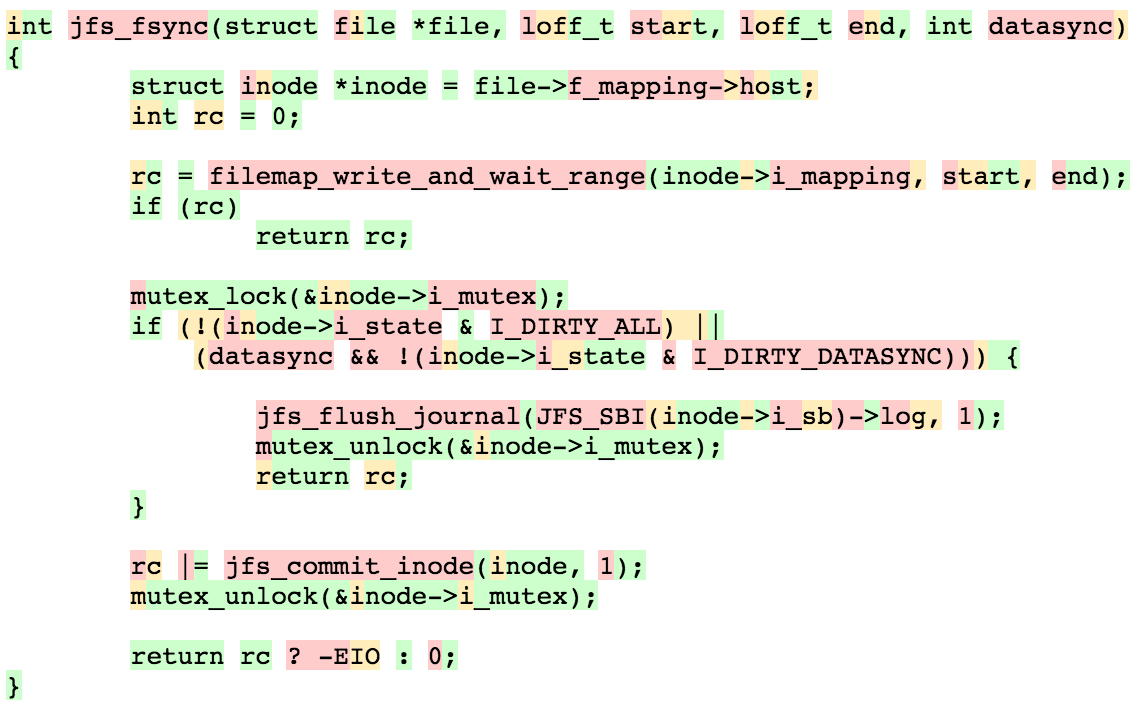
\includegraphics[width=\linewidth]{figs/code_example.png}
  \caption{Code example with per-character predictions}
  \label{fig:codeexample}
\end{figure}

